\chapter{Results}
By testing our implementation as described in section~\ref{sec:testing}, we verified that the program works as intended. Depressing a button caused the associated LED to light up. We also verified that the GPIO interrupts are fired correctly and only once per button press, and once per button raise.

\section{Energy usage}
A large focus of the exercise was energy efficiency. Our implementation used a current of 1.3$\mu$A when idle (i.e. no buttons being pressed).

We tested the four available drive strengths for the LED GPIO pins. The current with a single button depressed for various drive strengths is given in table~\ref{tbl:current}. In addition to getting different current readings, the intensity of the LEDs also differed. While the drive strength \texttt{LOWEST} gave a very weak light output, the three remaining were all bright enough for general use. We therefore decided on using the \texttt{LOW} setting, in the spirit of energy efficiency.

One surprising result is the 125$\mu$A current excluding the LED when using the \texttt{LOWEST} drive strength. We offer no explanation of why this happens, but assume it is an intricacy of the development kit.

\begin{table}
\centering
\begin{tabular}{ c c c }
  Drive strength & Current ($\mu$A) & Current including LEDs (mA) \\
  \hline
  LOWEST & 125 & 0.625 \\
  LOW & 80 & 7.0 \\
  STANDARD & 80 & 11.2 \\
  HIGH & 80 & 12.5
\end{tabular}
\caption{Current as measured by the AEM with one button depressed.}
\label{tbl:current}
\end{table}

\begin{figure}
\centering
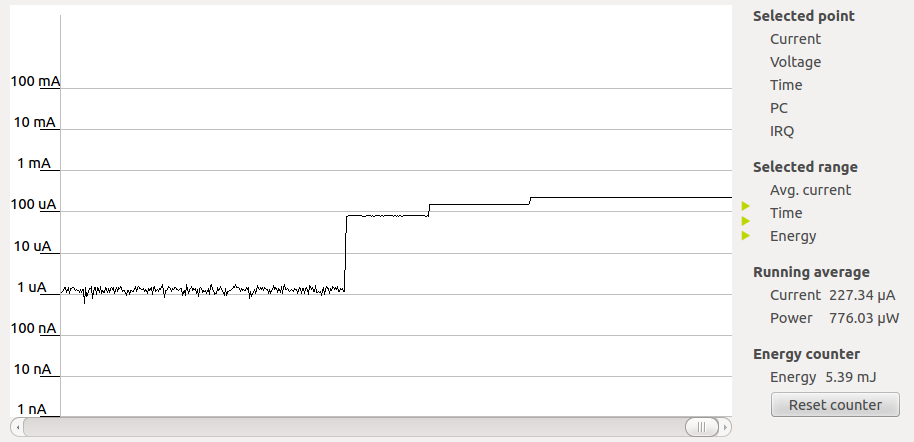
\includegraphics[width=\textwidth]{images/eaprofiler.png}
\caption{A screenshot from the eAProfiler program, showing current when idle and 1, 2 and 3 buttons are depressed.}
\end{figure}